\documentclass[14pt]{article}

\usepackage[cm]{fullpage}
\usepackage{fancyhdr}
\usepackage{setspace}

\usepackage[xetex]{graphicx}
\usepackage{fontspec,xunicode}
\defaultfontfeatures{Mapping=tex-text,Scale=MatchLowercase, Numbers=OldStyle}
\setmainfont[Scale=1]{Linux Libertine O}
\setsansfont{Linux Biolinum O}
\setmonofont{Monaco}

\usepackage{wrapfig}

\pagestyle{fancy}
\lhead{Phil Yeeles}
\rhead{\today}

\setlength{\headsep}{1.25cm}
\setlength{\parindent}{0cm}
\setlength{\parskip}{0.25cm}

\begin{document}

\begin{center}

{\LARGE {\bf \emph{Nico}: An Environment for Mathematical Expression in Schools}}

\end{center}

Thank you for agreeing to participate in the user study for my Part II Project!
\emph{Nico} is a piece of educational software designed to aid learners in the
visualisation of mathematical problems, by separating out the constituent parts
of a calculation into distinct units on-screen.

The purpose of this study is to ascertain how well \emph{Nico} achieves its goal
of providing a clear, accessible, interactive means of calculation, and to gather
feedback on how the application could be improved, by means of a few short
exercises.  Let us begin.

\section*{Welcome to \emph{Nico}!}

\subsection*{Introduction}

\emph{Nico} works by representing the constituent parts of a calculation as
circles containing an operator with arguments orbiting it.  The value of a circle
can be passed to other circles to be used in further calculations, and this is
indicated on-screen by means of a line going from from the edge of the argument
circle to the centre of the circle using it (\emph{Fig. 1}).

\begin{figure}[htb]
\centering
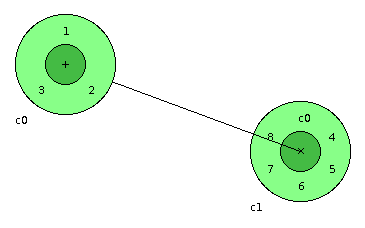
\includegraphics[scale=0.75]{fig1.png}
\caption{Nested circles, representing the calculation \emph{(1+2+3)×4×5×6×7×8}.}
\end{figure}

As the user builds up a diagram, the {\bf {\sffamily Answer}} field in the top
right-hand corner keeps a running total of the calculation, evaluating the circle
that does not use any others as arguments as the root.  Mousing-over a circle
currently in the diagram highlights that circle, and the relevant part of the
{\bf {\sffamily Question}} field that it represents, in blue.

\subsection*{Usage}

Begin by executing either the \verb¬nico¬ (for UNIX-like systems) or
\verb¬nico.bat¬ (for Microsoft Windows systems) file to open the application.
Upon opening the application, you will be presented with a file-chooser dialogue.
Use this to choose a set of questions (a file ending in \verb¬.nqs¬) to complete
using \emph{Nico}.

You are then presented with a screen akin to the one below (\emph{Fig. 2}).

\begin{figure}[!htb]
\begin{minipage}[b]{0.5\linewidth}
\centering
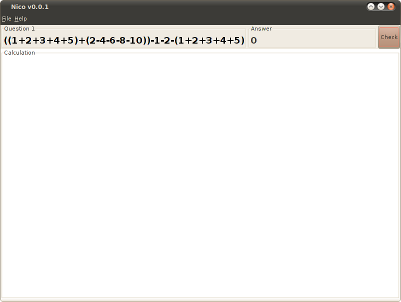
\includegraphics[scale=0.75]{fig2.png}
\caption{The initial state of the application upon loading a new question set.}
\end{minipage}
\hspace{0.5cm}
\begin{minipage}[b]{0.5\linewidth}
\centering
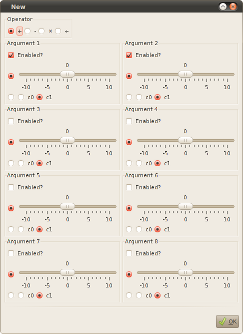
\includegraphics[scale=0.75]{fig3.png}
\caption{The dialogue box used for creating a new circle.}
\end{minipage}
\end{figure}

To create a circle, right-click on a blank section of the canvas.  A context menu
will appear, with a {\bf {\sffamily New circle}} option.  Select this option, and
you will be presented with a dialogue box, as depicted in \emph{Fig. 3}.

This dialogue box allows one to initialise a circle with up to eight arguments.
The operator is chosen with the radio buttons in the {\bf {\sffamily Operator}}
field.  The arguments are then set using the {\bf {\sffamily Argument}} fields.
Click on the {\bf {\sffamily Enabled?}} checkbox to use that argument in the
circle.  Choose either the radio button next to the slider or next to the list
of existing circles to specify whether the argument should be a number or
another circle.  If you select the slider, set the slider to the number (limited
to a minimum of -10 and a maximum of 10) you wish to use.  If you select the
list of existing circles, choose the radio button next to the label corresponding
to the circle that you wish to use.  Finally, click on the {\bf {\sffamily OK}}
button to create your circle.

You can add other circles as extra arguments by left-clicking and dragging between
the two circles: from the circle you wish to use to the circle you wish to use it
in.  To remove a circle, simply right-click on a circle and select
{\bf {\sffamily Remove circle}}.  Circles can be repositioned by left-clicking on
a circle and dragging it to the desired new position.

To check your answer, click the {\bf {\sffamily Check}} button in the top right-
hand corner of the window.  If the answer is correct, the {\bf {\sffamily Answer}}
text will turn green, a congratulatory message will pop up, and \emph{Nico} will
move on to the next question.  If your answer is incorrect, the
{\bf {\sffamily Answer}} text will turn red, and you will have the opportunity
to resubmit.

\section*{Exercises}

\begin{enumerate}

\item Open \emph{Nico} by executing the appropriate file for your system (either
\verb¬nico¬ or \verb¬nico.bat¬).  Open the question set
\verb¬user-study.nqs¬, which is in the subdirectory \verb¬qs/¬ of the main
application directory.

\item Work through the ten questions in the question set.

\item On completion of the question set, you will be presented with
another file-chooser dialogue.  Close this, and exit the application.

\item Complete the following questions (and please show your working!):--

\begin{enumerate}

\item \emph{2+3}\\

\fbox{
\begin{minipage}{16cm}
\hfill\vspace{3cm}
\end{minipage}
}\\

\pagebreak

\item \emph{9÷3}\\

\fbox{
\begin{minipage}{16cm}
\hfill\vspace{3cm}
\end{minipage}
}\\

\item \emph{1+2+3+4+5}\\

\fbox{
\begin{minipage}{16cm}
\hfill\vspace{3cm}
\end{minipage}
}\\

\item \emph{(2×4)+(3-5)}\\

\fbox{
\begin{minipage}{16cm}
\hfill\vspace{3cm}
\end{minipage}
}\\

\item \emph{((3×4)÷(3+3))×8}\\

\fbox{
\begin{minipage}{16cm}
\hfill\vspace{3cm}
\end{minipage}
}\\

\item \emph{((1+2+3+4+5)+(2×4×6×8×10))×1×2×(1+2+3+4+5)}\\

\fbox{
\begin{minipage}{16cm}
\hfill\vspace{3cm}
\end{minipage}
}\\

\pagebreak

\item \emph{12+14}\\

\fbox{
\begin{minipage}{16cm}
\hfill\vspace{3cm}
\end{minipage}
}\\

\item \emph{247×35}\\

\fbox{
\begin{minipage}{16cm}
\hfill\vspace{3cm}
\end{minipage}
}\\

\item \emph{120÷((2×10)+5+5)}\\

\fbox{
\begin{minipage}{16cm}
\hfill\vspace{3cm}
\end{minipage}
}\\

\item \emph{((2+5)×(6÷2)×(9-8))+((3+4)-(5×6))+120}\\

\fbox{
\begin{minipage}{16cm}
\hfill\vspace{3cm}
\end{minipage}
}\\

\end{enumerate}

\item Fill out the feedback section below.

\end{enumerate}

\section*{Feedback}

% is it intuitive?
% is it easy to use?
% is it clear what the syntax means?
% is it any better than just doing maths on paper?
% what could be improved?
% any other thoughts?



\begin{enumerate}

\item Please circle on the scale below how easy-to-use you felt \emph{Nico}
was.

\begin{center}
{\Huge \vspace{-0.5cm}☹\hspace{0.25cm}{\bf ·}\hspace{0.25cm}{\bf ·}\hspace{0.25cm}{\bf ·}\hspace{0.25cm}☺\\}
\end{center}

\item Please circle on the scale below how intuitive you found using \emph{Nico}
to be.

\begin{center}
{\Huge \vspace{-0.5cm}☹\hspace{0.25cm}{\bf ·}\hspace{0.25cm}{\bf ·}\hspace{0.25cm}{\bf ·}\hspace{0.25cm}☺\\}

\end{center}

\pagebreak

\item Did you prefer working with \emph{Nico} to working the answers out on
paper (circle as appropriate)?

\begin{center}
Yes\hspace{1cm}No\\
\end{center}

\fbox{
\begin{minipage}{17cm}
Why?\hfill\vspace{2cm}
\end{minipage}
}\\

\item Please circle on the scale below how clearly you felt the circle notation
illustrated the flow of information throughout the calculation.

\begin{center}
{\Huge \vspace{-0.5cm}☹\hspace{0.25cm}{\bf ·}\hspace{0.25cm}{\bf ·}\hspace{0.25cm}{\bf ·}\hspace{0.25cm}☺\\}
\end{center}

\item How could \emph{Nico} be improved?  Would you add any features?  Would you
take any features away?\\

\fbox{
\begin{minipage}{17cm}
\hfill\vspace{3cm}
\end{minipage}
}\\

\item Any other thoughts?\\

\fbox{
\begin{minipage}{17cm}
\hfill\vspace{3cm}
\end{minipage}
}\\

\end{enumerate}

Thank you very much for your help with my project!  Your responses will remain
confidential, although they are liable to appear in the final report, of which a
copy will be retained by the University of Cambridge Computer Laboratory Library\\
(\verb¬http://www.cl.cam.ac.uk/library/¬).  The final report will also be
available via my repository at GitHub\\
(\verb¬http://github.com/loomcore/nico¬).

\begin{center}

\fbox{
\parbox{18cm}{
\begin{center}
{\large {\bf Declaration}}\\\vspace{0.5cm}
I hereby authorise the use of my responses to this study in the author's Part II
Project for the University of Cambridge Computer Science Tripos.  I acknowledge
that my responses may be published in the final report, and that this report will
be made publicly available from the Univeristy of Cambridge Computer Laboratory
Library and from GitHub.\\
\end{center}
\begin{spacing}{2}
{\bf Signed:}
\end{spacing}
\begin{spacing}{1.5}
{\bf Name:}\\
{\bf Date:}\\
\end{spacing}
}
}

\end{center}

\end{document}
